\section{The Liquid Crystalline phase of matter} 

As one may expect from the name, the \textit{liquid crystalline} phase is a curious state of matter that lies somewhere between the \textit{solid crystalline} and the \textit{isotropic fluid} phases. As such, the liquid crystalline phase can exhibit extraordinary properties that belong to both the solid crystalline and isotropic fluid states of matter individually. For example, a liquid crystal can be shown to have the freedom to flow like any ordinary liquid (characteristic of the fluid phase) but also have the ability to exhibit birefringence (a characteristic of the solid crystalline phase). For such an exotic `fourth state of matter', the term \textit{mesophase} or \textit{mesomorphic phase} is coined, meaning, quite simply, \textit{intermediate phase} \citep{Vertogen1988}. 

Crudely speaking, all mesophases can be said to fall into one of two sub categories,

\begin{enumerate}
	\item \textit{Thermotropic} liquid crystals - the liquid crystalline mesophase occurs within a specific temperature range.
	\item \textit{Lyotropic} liquid crystals - the liquid crystalline mesophase occurs within a specific concentration range when dissolved in a solvent solution. Interestingly, many common materials show lyotropic behaviour, perhaps most importantly the bilayer membranes of living cells, where theories developed for liquid crystal physics have helped shed light on the effect of mitosis \citep{Lydon2006}. Perhaps less importantly, lyotropic materials are also mass produced for products such as shampoo and ice cream \cite{Taphouse2007}.
\end{enumerate}

Display devices, arguably the driving force behind the majority of liquid crystal research, are constructed solely from the thermotropic class of liquid crystal, and will therefore be the core study of this thesis.

\subsection{Thermotropic liquid crystals}
\label{sec:Thermotropic_liquid_crystals}
As is often the case when an area of science unites Physics, Chemistry and Biology, a multitude of classifications and labels are used to define subsets of materials. Liquid crystal classification is no different, and as such, the thermotropic class of liquid crystals can be further divided into the subdivisions of \textit{Calamitic}, \textit{Discotic} and \textit{Polymeric}, where the division is made solely on the physical nature of the molecule comprising the liquid crystal phase.

\begin{itemize}
\item \textit{Calamitic} liquid crystals are constructed from long, rod-like (uniaxial) molecules (see Figure \ref{fig:5cb_molecule}). They exhibit a principal axis of orientation whereby the long molecular axes tend to align parallel to one another.
\item \textit{Discotic} liquid crystals are constructed from disc shaped molecules (one axis is significantly shorter that the other two) and tend to align by stacking on top of each other like coins.
\item \textit{Polymeric} liquid crystals are constructed from long chain polymer molecules.
\end{itemize}

\begin{figure}
\begin{center}
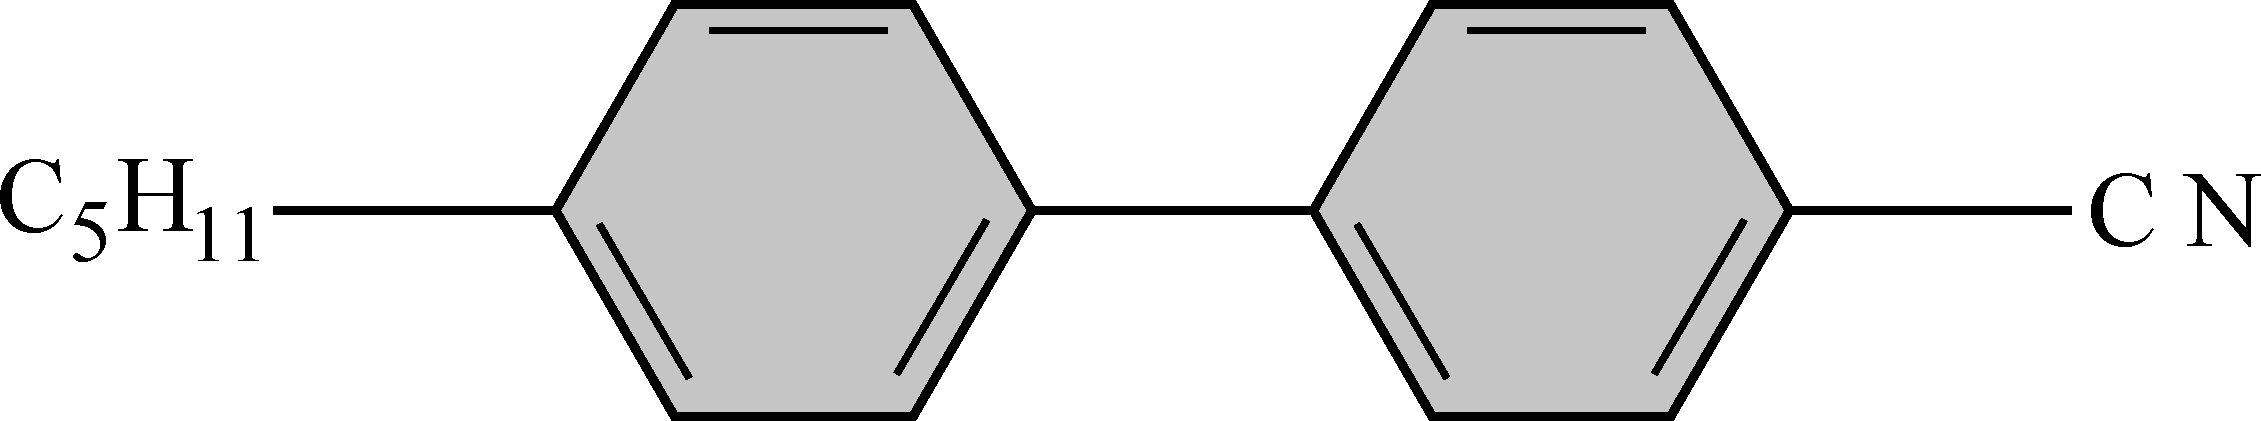
\includegraphics{figures/introduction/5CB_molecule.pdf}
\end{center}
\caption[The molecular structure of 5CB]{\label{fig:5cb_molecule} The molecular structure of 5CB. With one long and 2 short axes, 5CB is a calamitic or `rod like' material.}
\end{figure}

By far the majority of liquid crystal display devices are constructed from calamitic molecules, and through early work in the field, Friedel  \cite{Friedel1922} was able to show that the calamitic class of molecule can be further divided into three separate sets, \textit{Nematic}, \textit{Smectic} and \textit{Cholesteric} (see Figure \ref{fig:phases}). This time with the division made solely on the degree of order exhibited by the molecules in the phase.

\begin{itemize}
\item \textit{Nematic} molecules posses three translational degrees of freedom and exhibit short-range orientational order whilst the molecular centres are distributed at random.
\item \textit{Smectic} molecules exhibit a positional order in at least one dimension, with the molecular centres on average arranged in equidistant planes\footnote{There are many smectic phases, running from $S_A,S_B,...S_I$, differing in molecular orientation and layer spacing}.
\item \textit{Cholesteric} molecules are very similar to those of the nematic class, but possess a twist in the direction of the short-range order as a function of position in the sample. 
%Remembering the equivalence of $\bm{n}$ and $-\bm{n}$, the period of repetition is the helical pitch $p$ divided by 2.
\end{itemize}


\begin{figure}
\begin{center}
\subfigure[Isotropic fluid]{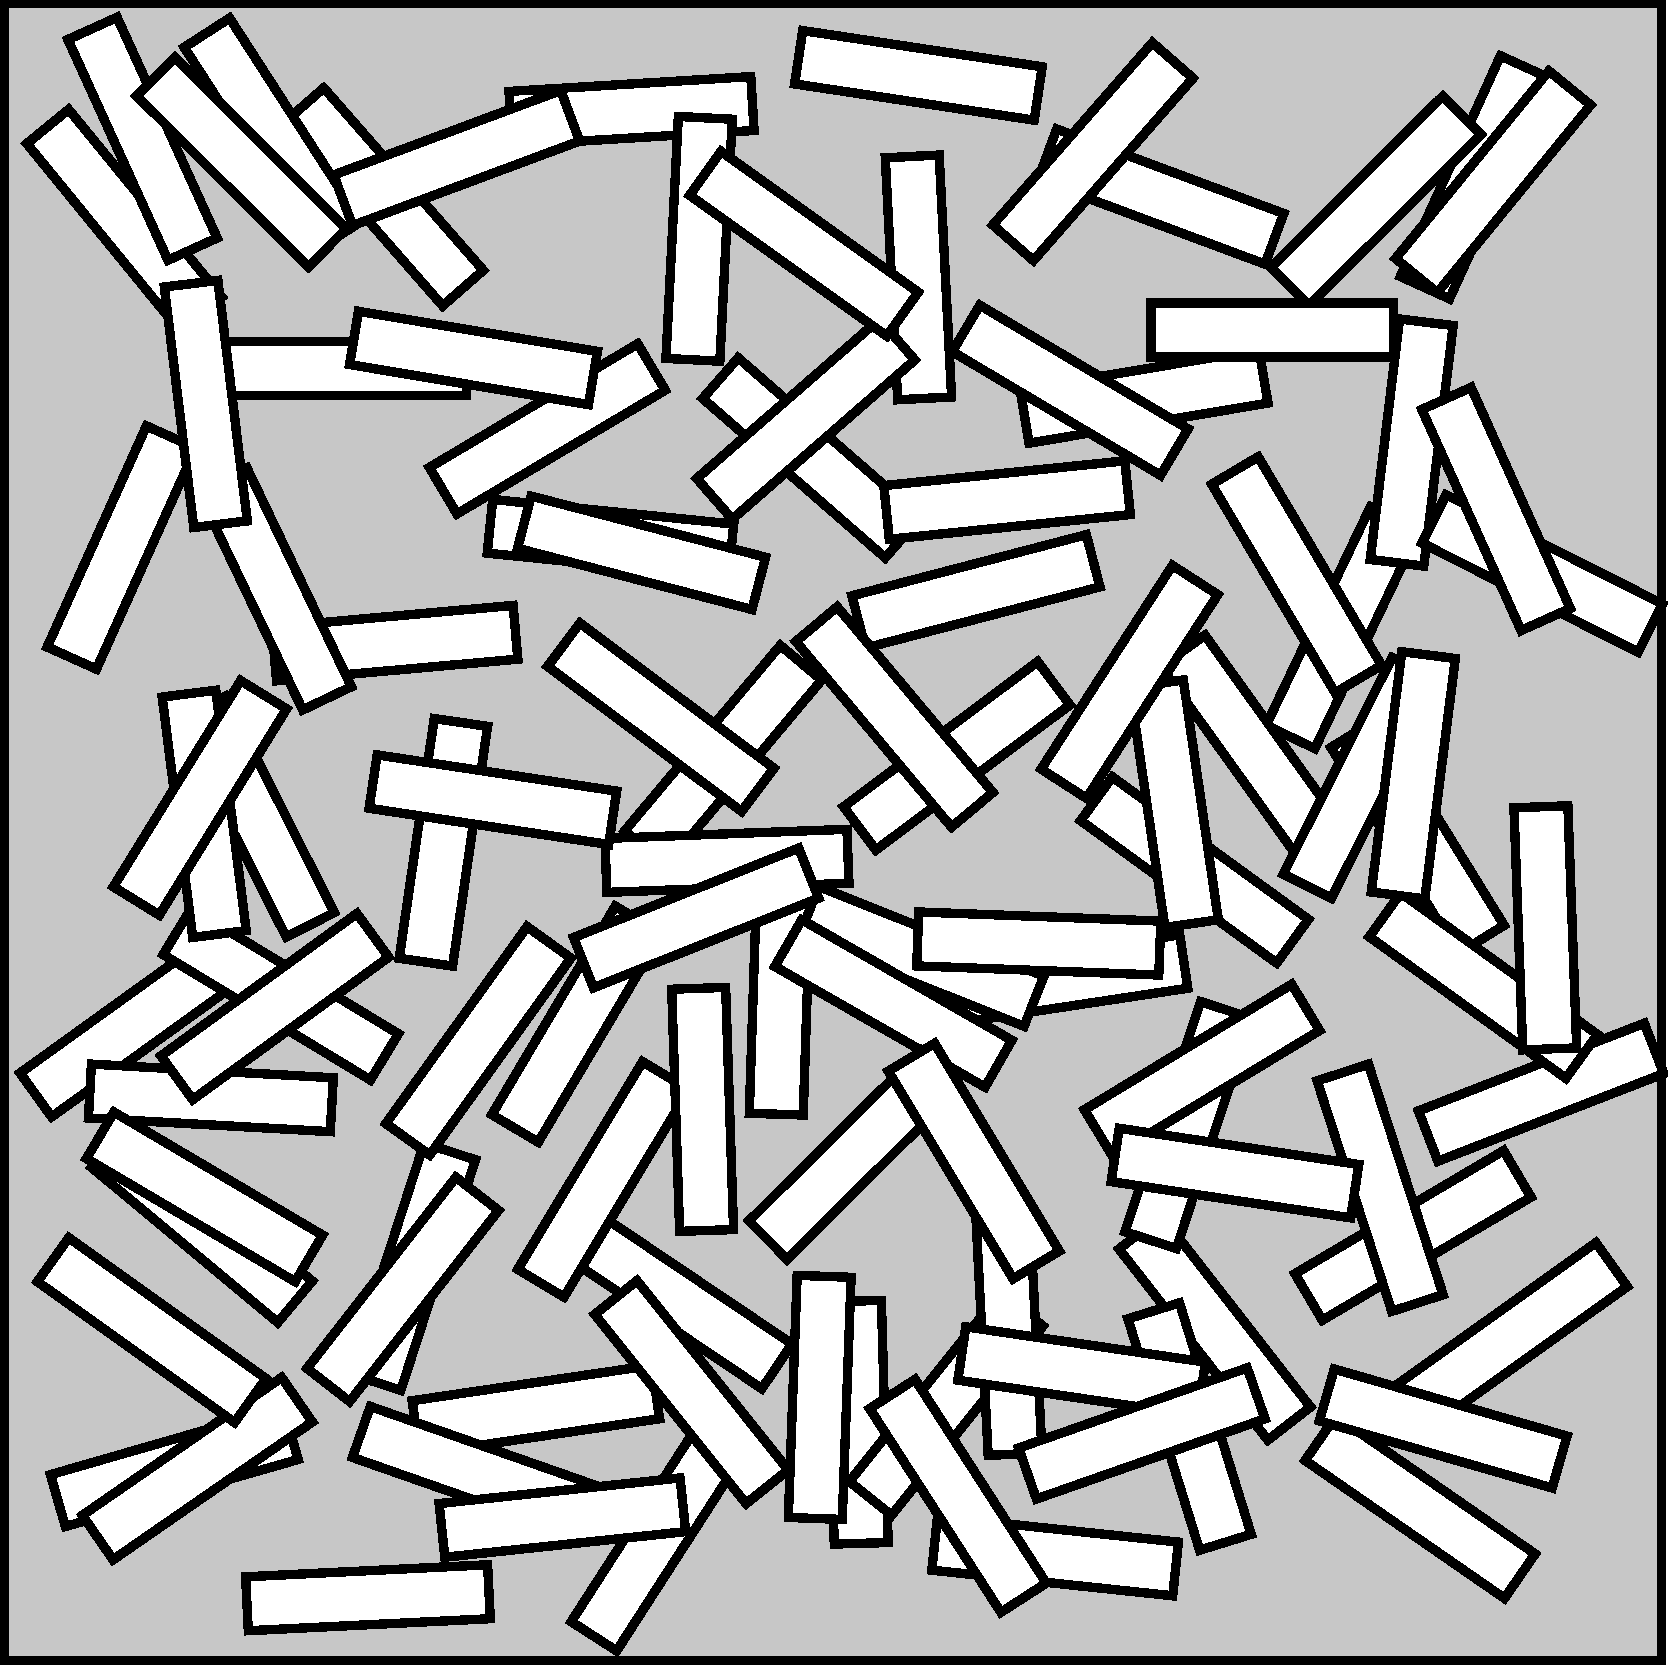
\includegraphics[width=0.2\textwidth]{figures/introduction/isotropic_phase}}\hspace{0.5cm}
\subfigure[Nematic phase]{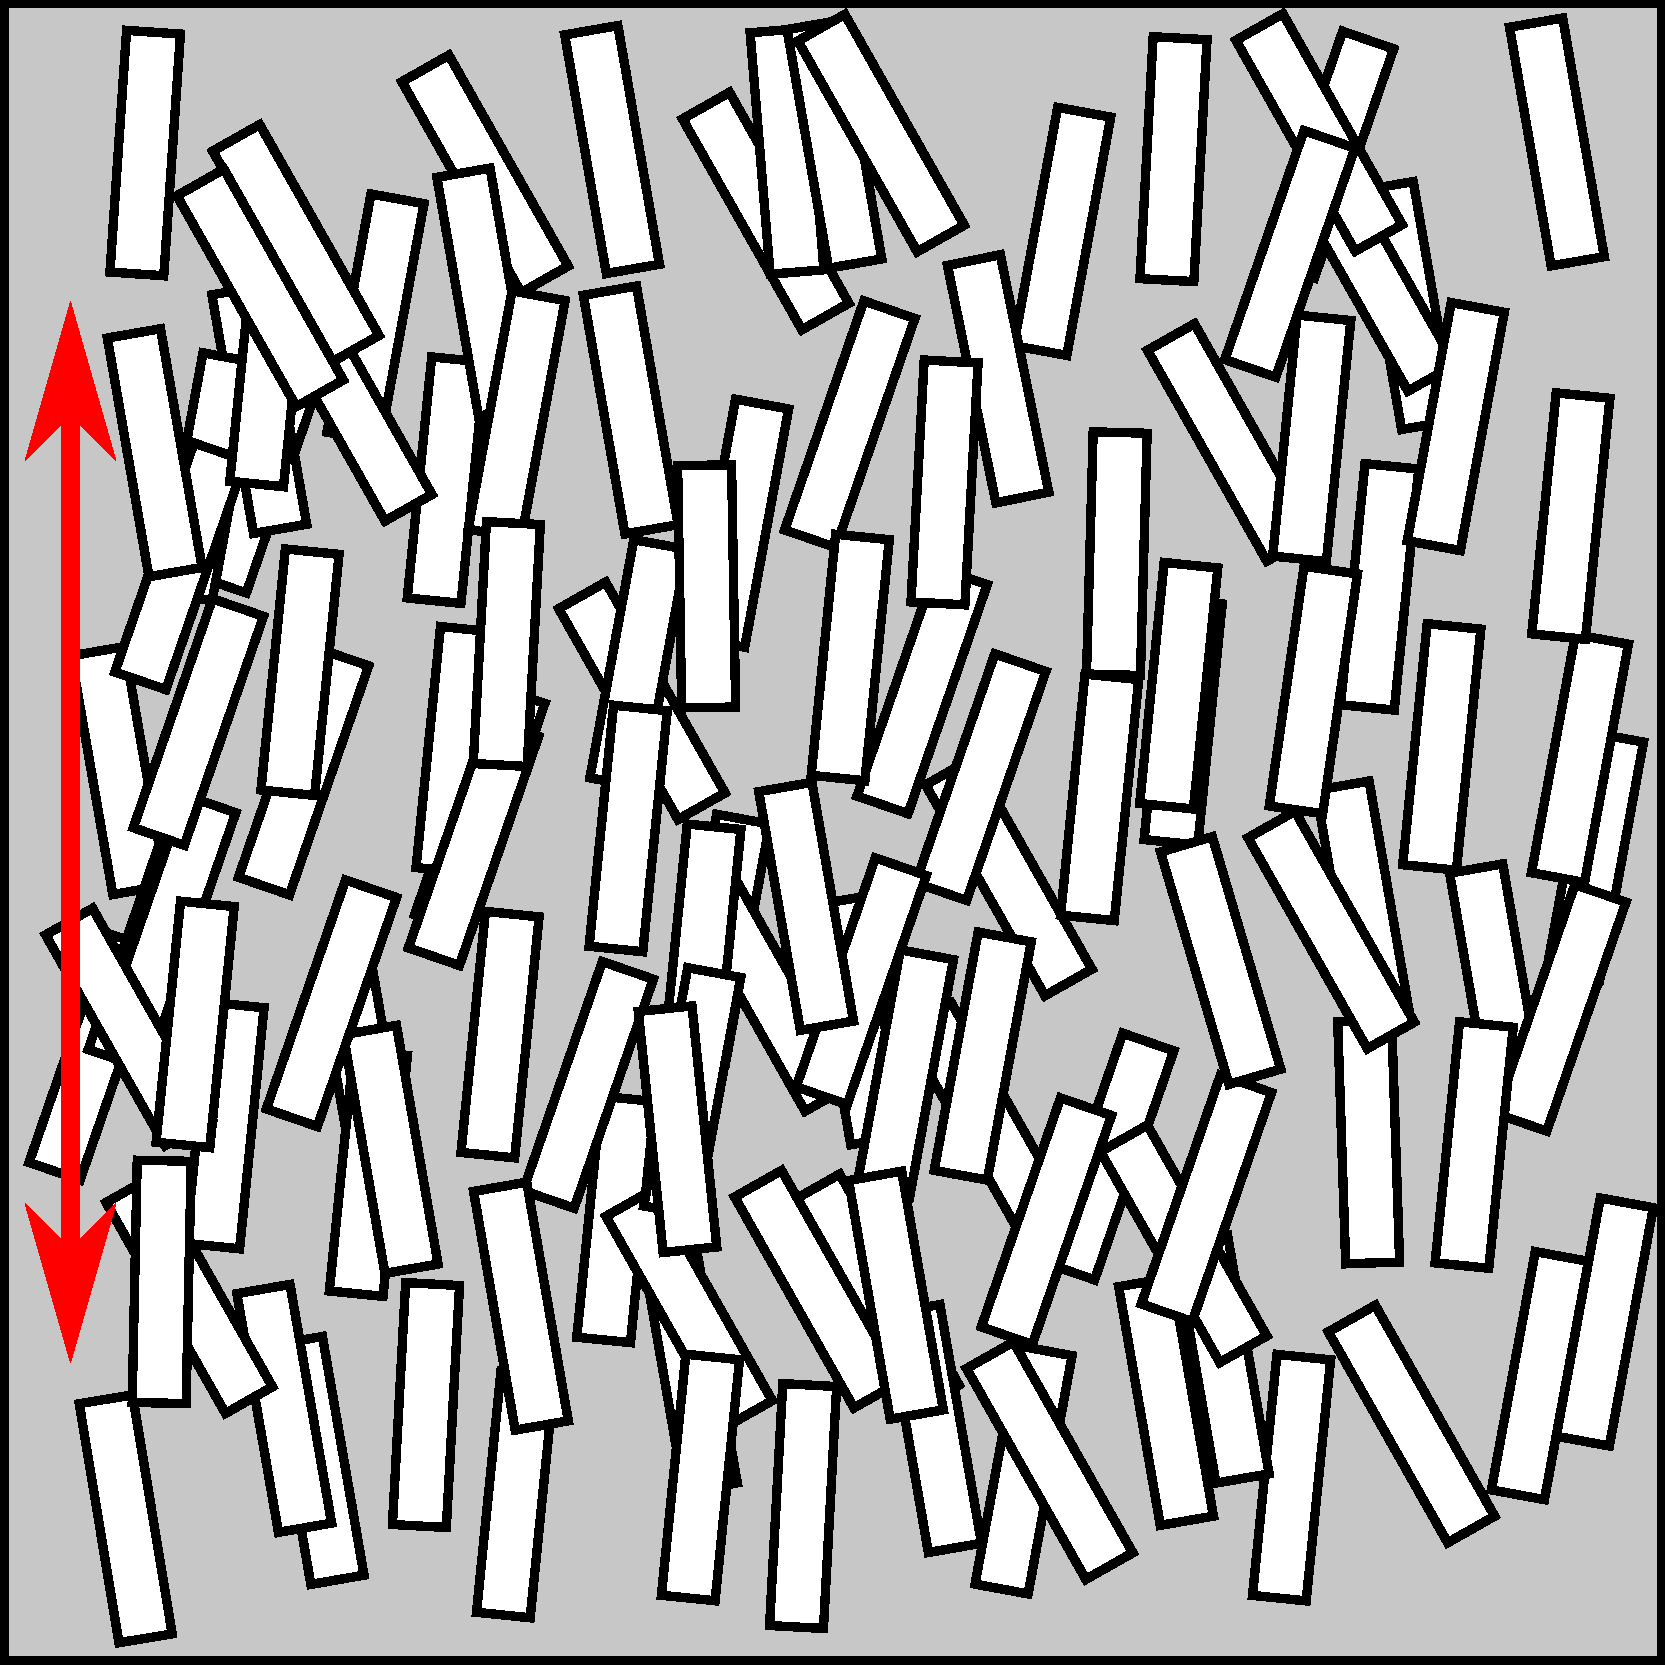
\includegraphics[width=0.2\textwidth]{figures/introduction/nematic_phase}}\hspace{0.5cm}
\subfigure[Smectic A phase]{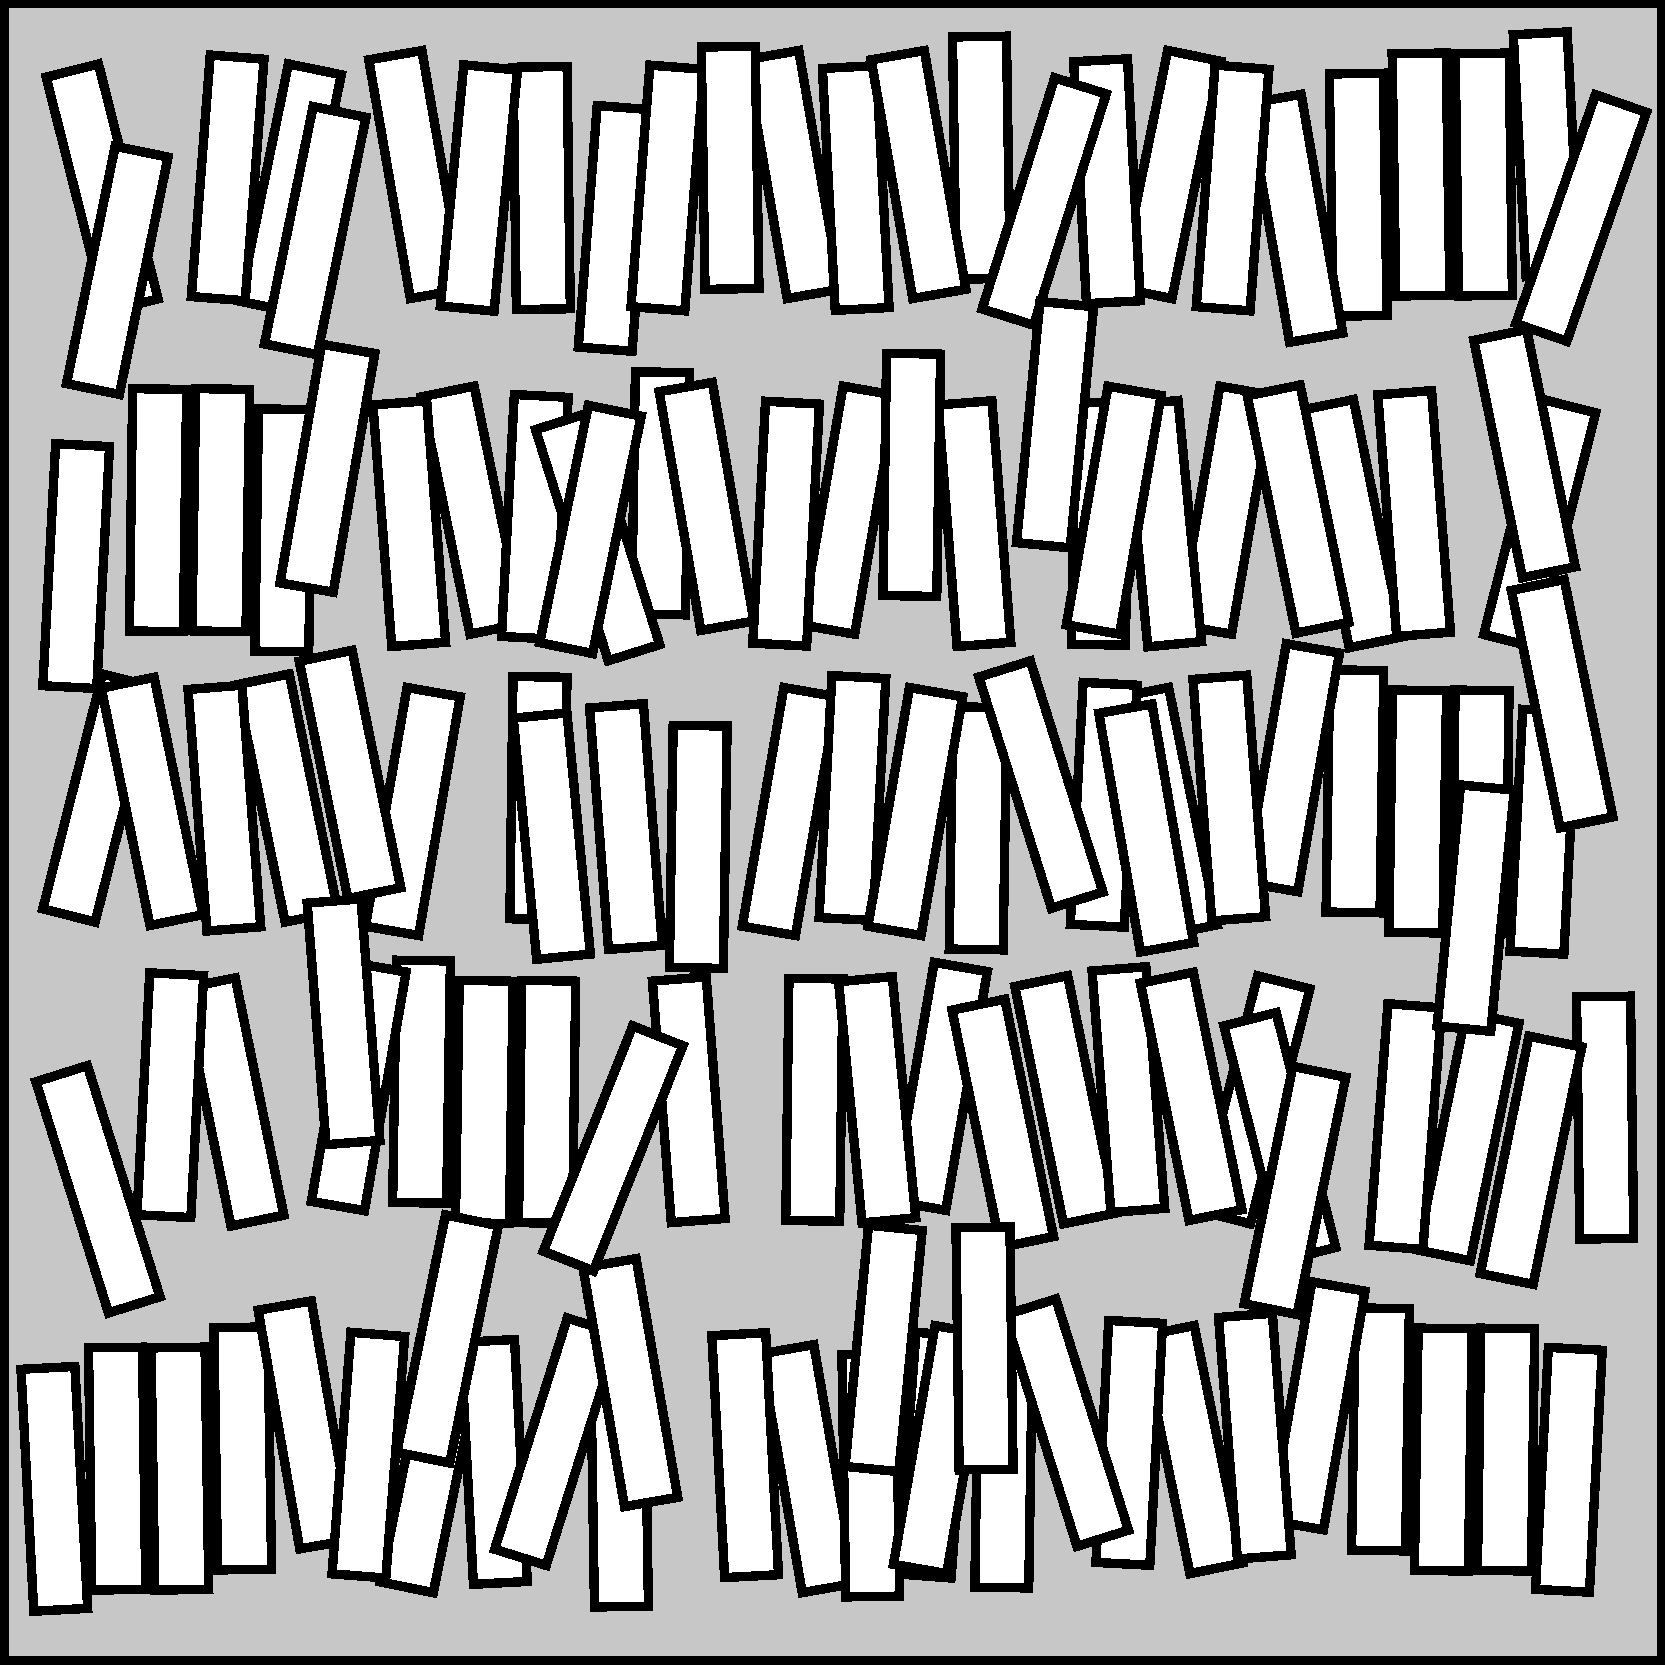
\includegraphics[width=0.2\textwidth]{figures/introduction/smectic_phase}}\hspace{0.5cm}
\subfigure[Solid Crystalline]{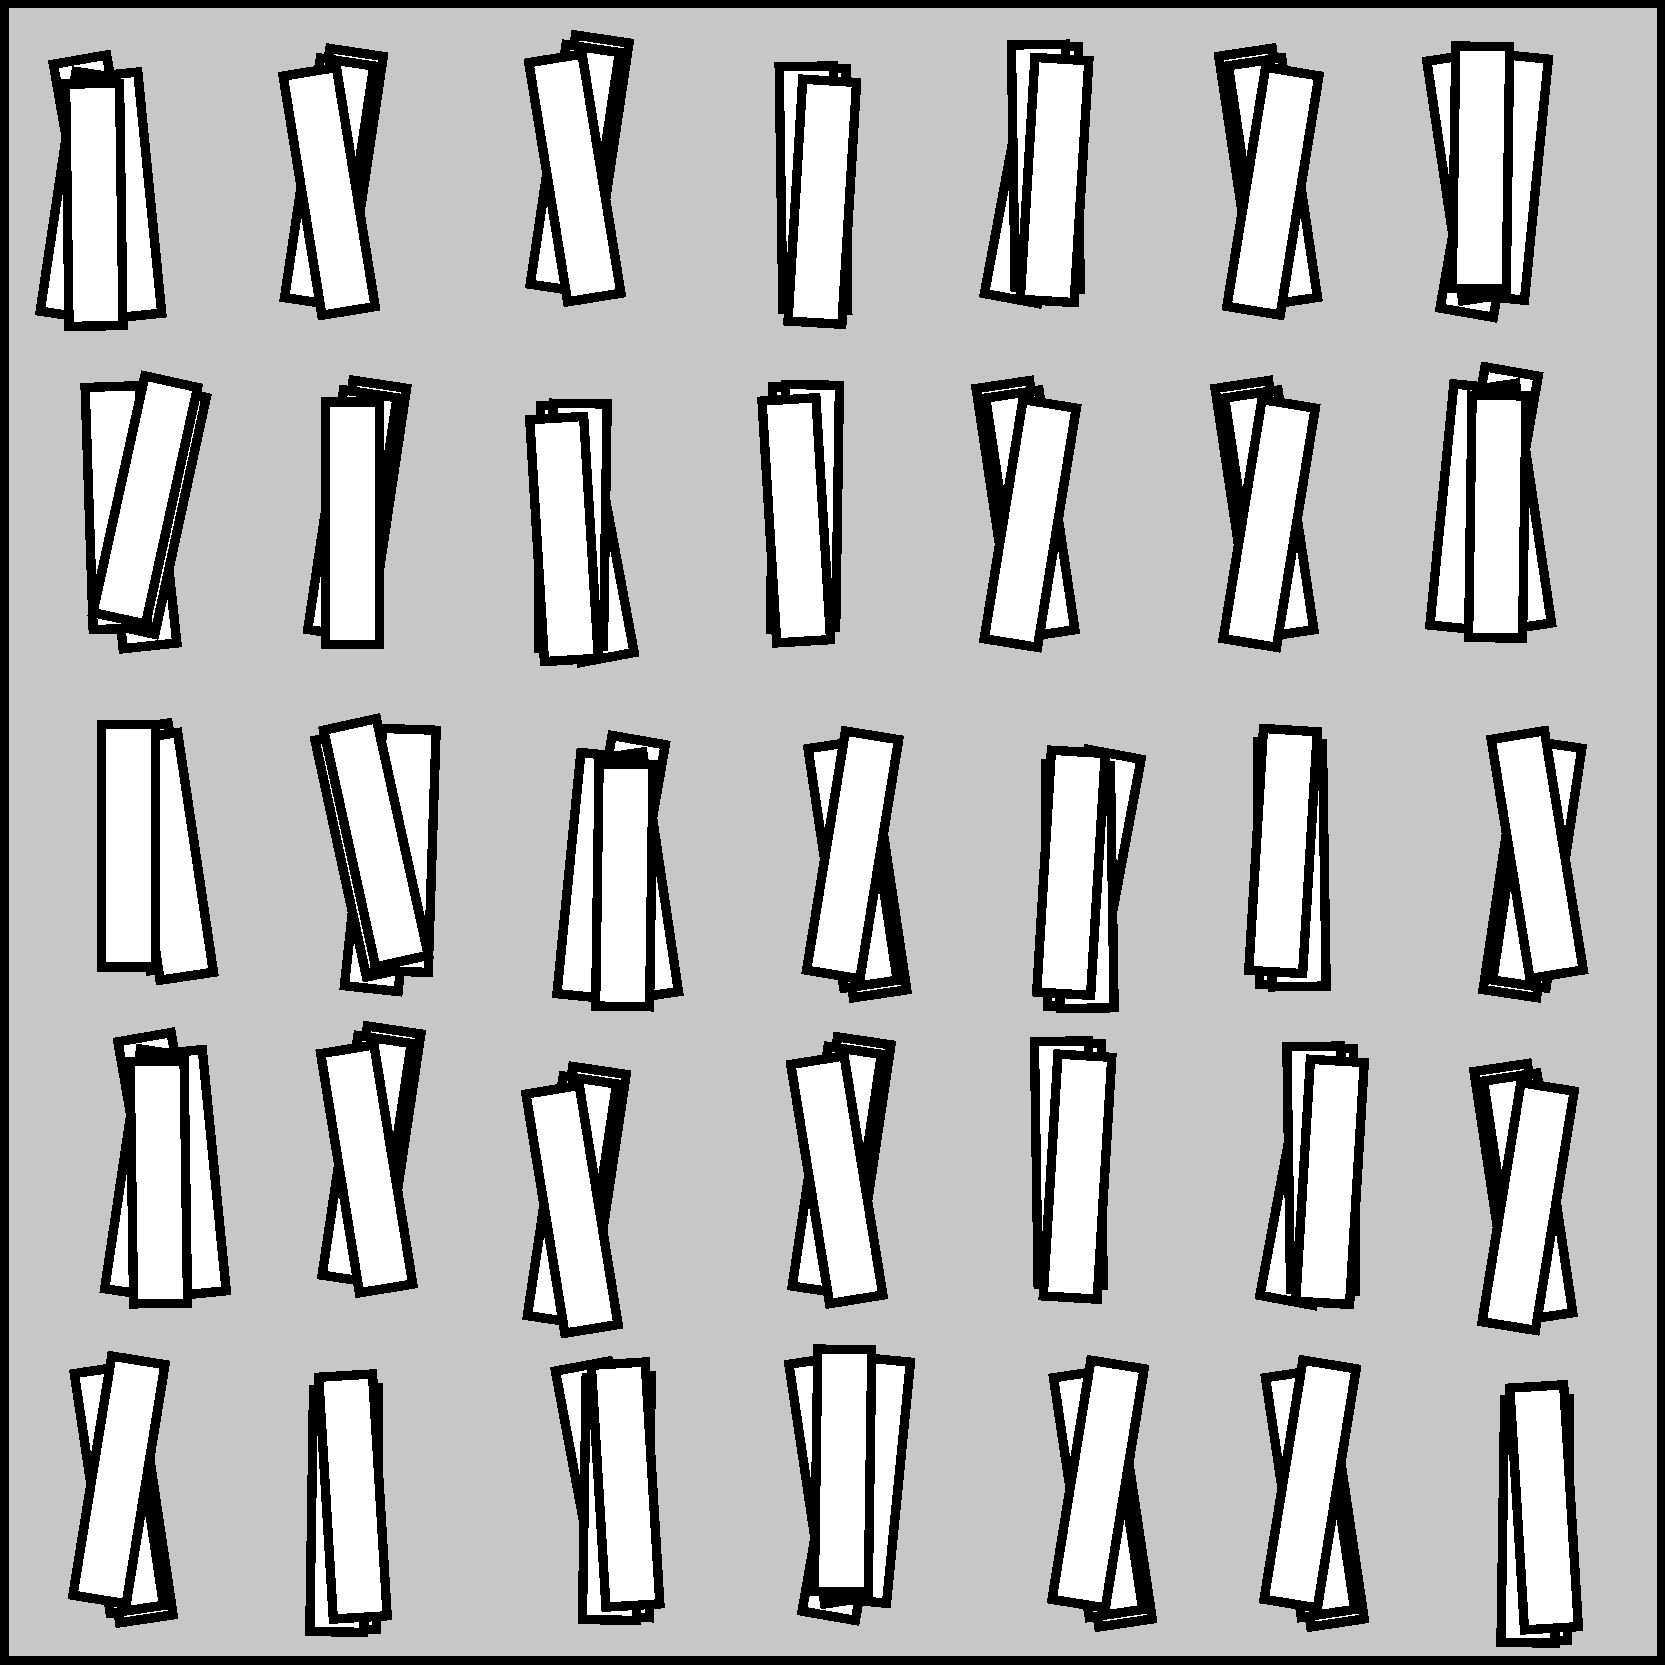
\includegraphics[width=0.2\textwidth]{figures/introduction/crystal_phase}}\hspace{0.5cm}
\end{center}
\caption[Schematic depiction of various liquid crystalline phases]{\label{fig:phases}Figures (a - d) depict schematic representations of the isotropic fluid, nematic, smectic and solid crystalline phases of matter. Each white rectangle represents an anisotropic molecule of the medium. The red arrow in (b) defines the average orientation of the molecules, known as the director.}
\end{figure}

This classification system for mesophases and their molecule type is summarised by the flow chart in Figure \ref{fig:flow_chart}.

\begin{figure}
\begin{center}
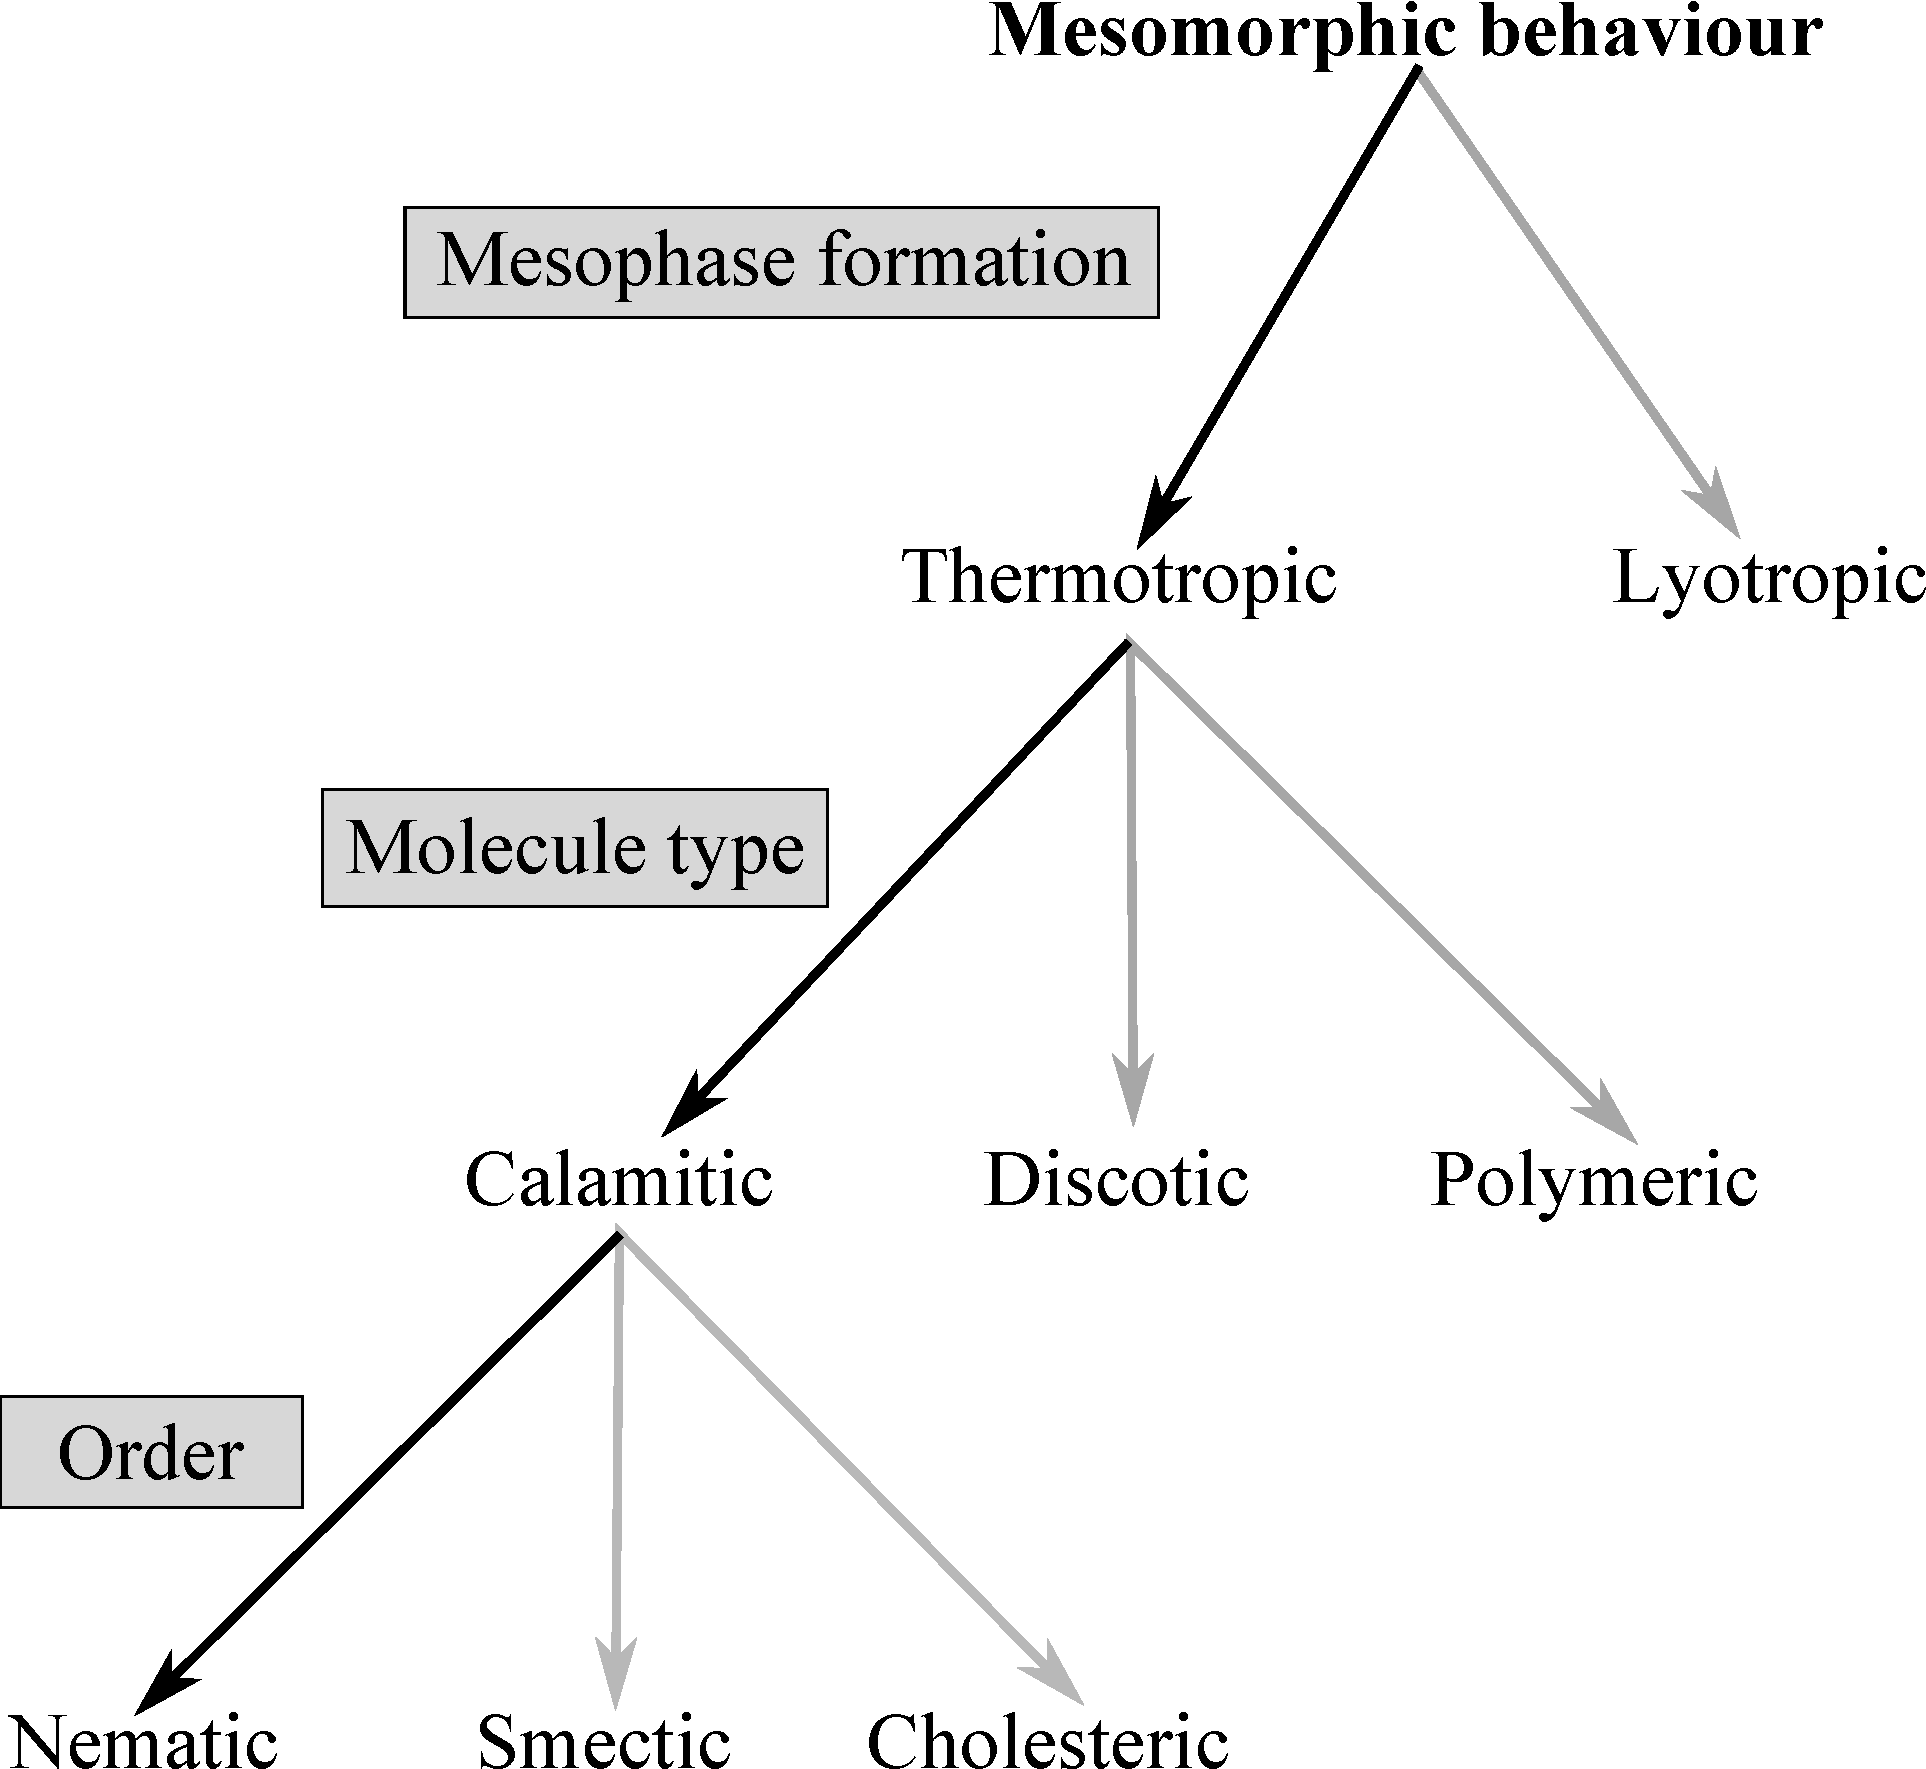
\includegraphics{figures/introduction/flow_chart.pdf}
\end{center}
\caption[Mesophase sub-division flow chart]{\label{fig:flow_chart}A flow chart summarising the sub-divisions of mesophases and the criteria upon which the subdivisions are made (grey boxes).}
\begin{center}
%\rule{3in}{0.5pt}
\end{center}
\end{figure}

\subsection{Nematic liquid crystals}
\label{sec:nematic_mesophase}
The main focus of the work in this thesis concerns the dynamic properties of nematic liquid crystals. As such, the features and properties that are key to understanding the nematic phase of thermotropic liquid crystals are summarised in the following paragraphs.

Firstly, included below are the three essential features exhibited by nematic phases,

\begin{itemize}
\item Nematic molecules will align, on average, with their long axes parallel to each other. Over macroscopic length scales, this alignment leads to a preferred direction in space, represented by \textit{the director} $\hat{\bm{n}}$. For almost all known thermotropic nematics, there exists rotational symmetry about $\hat{\bm{n}}$.
\item There is no correlation between the molecular centres of mass (no positional order). Hence the nematic phase is a fluid.
\item There is no polarity associated with the uniaxial axis of symmetry $\left(\hat{\bm{n}}=-\hat{\bm{n}}\right)$.
\end{itemize}

\subsection{Nematic Order}
The uniaxial, `rod like' molecules of a nematic liquid crystal are defined to have an \textit{ordinary} axis (denoted by a subscript $o$) with a length scale on the order of 5 \AA, and an \textit{extraordinary} axis (denoted by a subscript $e$) with a length scale on the order of 20 \AA. In addition to the uniaxiality of nematics, as mentioned in Section \ref{sec:nematic_mesophase}, the nematic phase also exhibits a degree of short-range orientational order. Over macroscopic length scales, the orientation of individual molecules in a distribution will vary slightly, and importantly, this variation can be considered as time dependent, due to thermal fluctuations in the environment.

As such, the orientational order of a macroscopic sample is quantified by the order parameter, $s$, of the system, a quantity between $s=0$ (random distribution of molecular orientations) and $s=1$ (all molecules parallel to the director)\citep{Collings1997}. The value of a system's order parameter can be calculated from

\begin{equation}
s=\left\langle \frac{3}{2}\cos^2\theta-\frac{1}{2}\right\rangle
\label{eq:Order}
\end{equation}

where $\theta$ is the angle between the individual molecule and the director, and the brackets denote an average taken over all molecules of the sample. In practice, the value of $s$ is normally found to be around 0.3 or 0.4 at the clearing point, $T_c$ (the transition temperature from the liquid crystal to isotropic fluid phase), and is found to be around 0.8 at much lower temperatures \citep{Vertogen1988}. 

\subsection{Optical Anisotropy}
The uniaxial shape of a nematic molecule results in the refractive index associated with light polarised parallel to the director $\left( n_{e}\right)$ differing from that of light polarised perpendicular to the director $\left(n_{o}\right)$. This fundamental difference in the refractive indices is termed the \textit{birefringence}, and is defined as
 
\begin{equation}
\Delta n=n_{e}-n_{o}
\end{equation}

It is this birefringence that is exploited in all liquid crystal displays to produce contrast between picture elements. The values of $n_o$ and $n_e$ will differ with incident wavelength and also change as a function of temperature. For the liquid crystal 5CB at 25 $^{\circ}$C and a wavelength of 633 nm, values of the refractive indices are close to $n_o=1.531$ and $n_e=1.706$ \cite{Li2005}. Simply, if one considers a nematic liquid crystal sample where the temperature is being increased (and therefore through thermal fluctuations the order parameter is decreasing) it is easy to see that $\Delta n$ will also decrease, and above $T_c$ the refractive index is clearly single valued.  

\subsection{Dielectric Anisotropy}
In direct parallel with the optical anisotropy, the dielectric permittivities are also directionally dependent, in association with the ordinary and extraordinary axes of the liquid crystal. The dielectric anisotropy is defined as,
\begin{equation}
\Delta\epsilon=\epsilon_{e}-\epsilon_{o}.
\end{equation}

The value of $\Delta\epsilon$ is responsible for dictating the reorientation of the director in response to an applied field. In the case of positive dielectric anisotropy ${\left(\epsilon_{e}>\epsilon_{o}\right)}$, the director will align parallel to the applied field lines. In the case of negative dielectric anisotropy ${\left(\epsilon_{e}<\epsilon_{o}\right)}$ the director will tend to align perpendicular to the field lines. It is this interaction between the reorientation of the director and the applied field, that is used to switch picture elements on and off in liquid crystal displays.

\subsection{Elastic Constants and Free Energy}
\label{sec:Elastics}
Due to spatial variations in the director, a nematic liquid crystal will always exhibit elastic free energy. When the director profile is confined between two aligning boundary layers, the molecules will reorientate to minimise the free energy per unit volume. As such, an appropriate free energy density $w_f$ is defined by Frank and Oseen.

\begin{equation}
w_f=\frac{1}{2}k_{11}\left(\nabla.\bm{n}\right)^2+\frac{1}{2}k_{22}\left(n.\nabla.\times\bm{n}\right)^2+\frac{1}{2}k_{33}\left|\bm{n}\times\nabla\times\bm{n}\right|^2
%+\frac{1}{2}\left(k_{22}+k_{24}\right)\nabla.\left(\bm{n}.\nabla\bm{n}-\bm{n}\nabla.\bm{n}\right)
\label{eq:Free_energy}
\end{equation}

Here, the constants $k_{11},k_{22}$ and $k_{33}$ correspond to the elastic deformations of the director field, splay, twist and bend, as are pictorially demonstrated in Figure \ref{fig:s,t,b}. For typical nematic liquid crystals, the elastic constants have values on the order of $10^{-11}$ N, which are obtained from experiments involving the competing effects of surface alignment and applied field alignment \citep{Vertogen1988}. Typical values for the liquid crystal 5CB are given as $k_{11}=0.62\times10^{-11} \text{ N},k_{22}=0.39\times10^{-11} \text{ N}\text{ and }k_{33}=0.82\times10^{-11} \text{ N}$ \cite{Stewart2004}. In the case of chiral nematics, a fourth term is added to the expression for the free energy density,

\begin{figure}
\begin{center}
\subfigure[Splay]{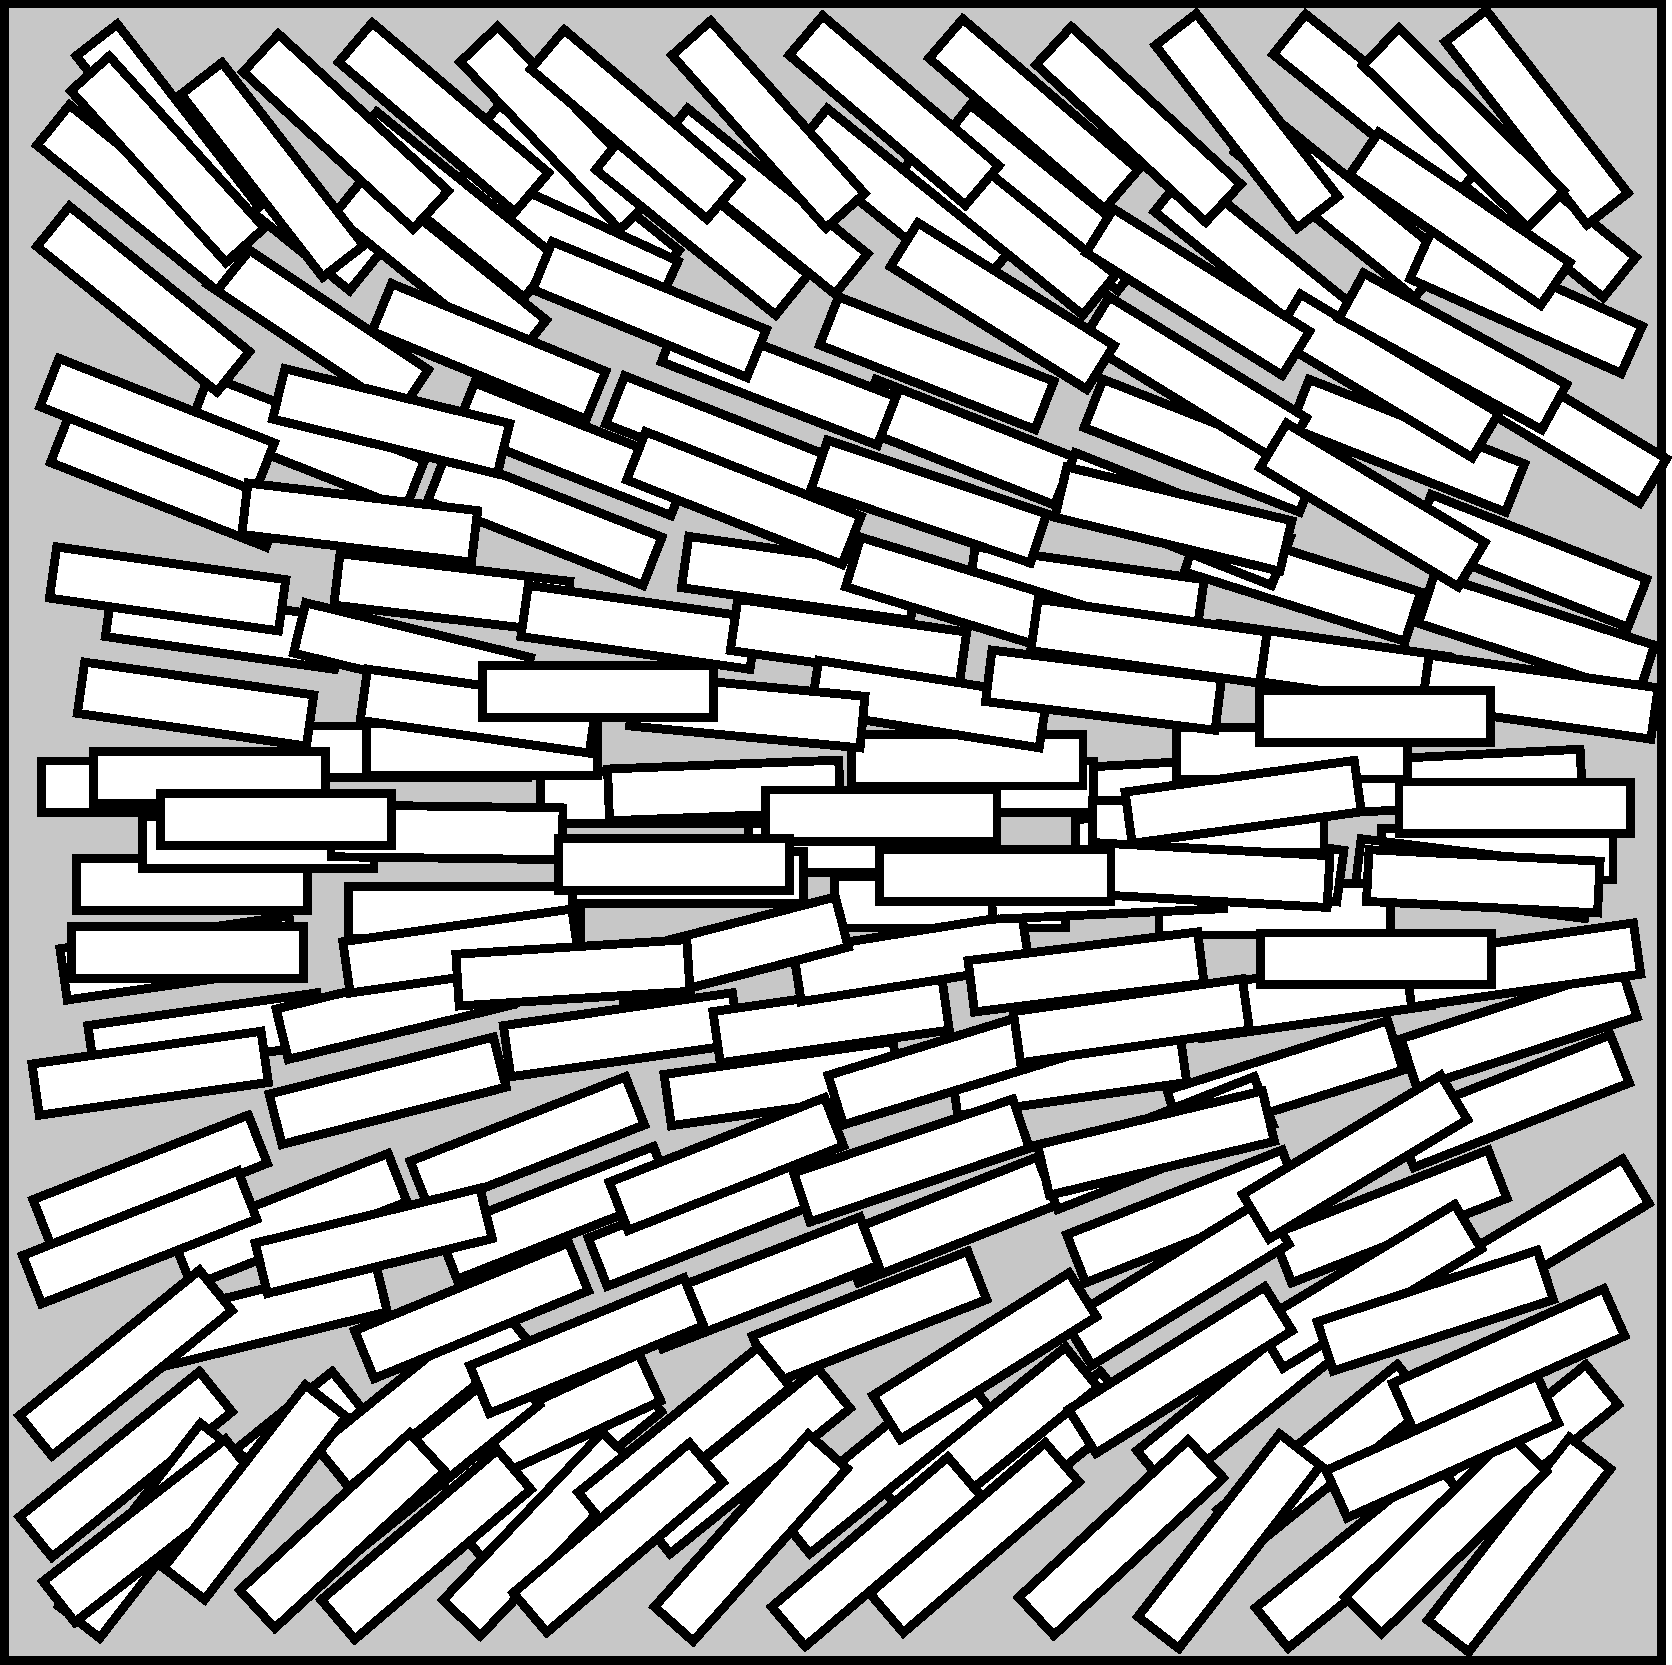
\includegraphics[width=0.2\textwidth]{figures/introduction/splay}}\hspace{0.2cm}
\subfigure[Twist]{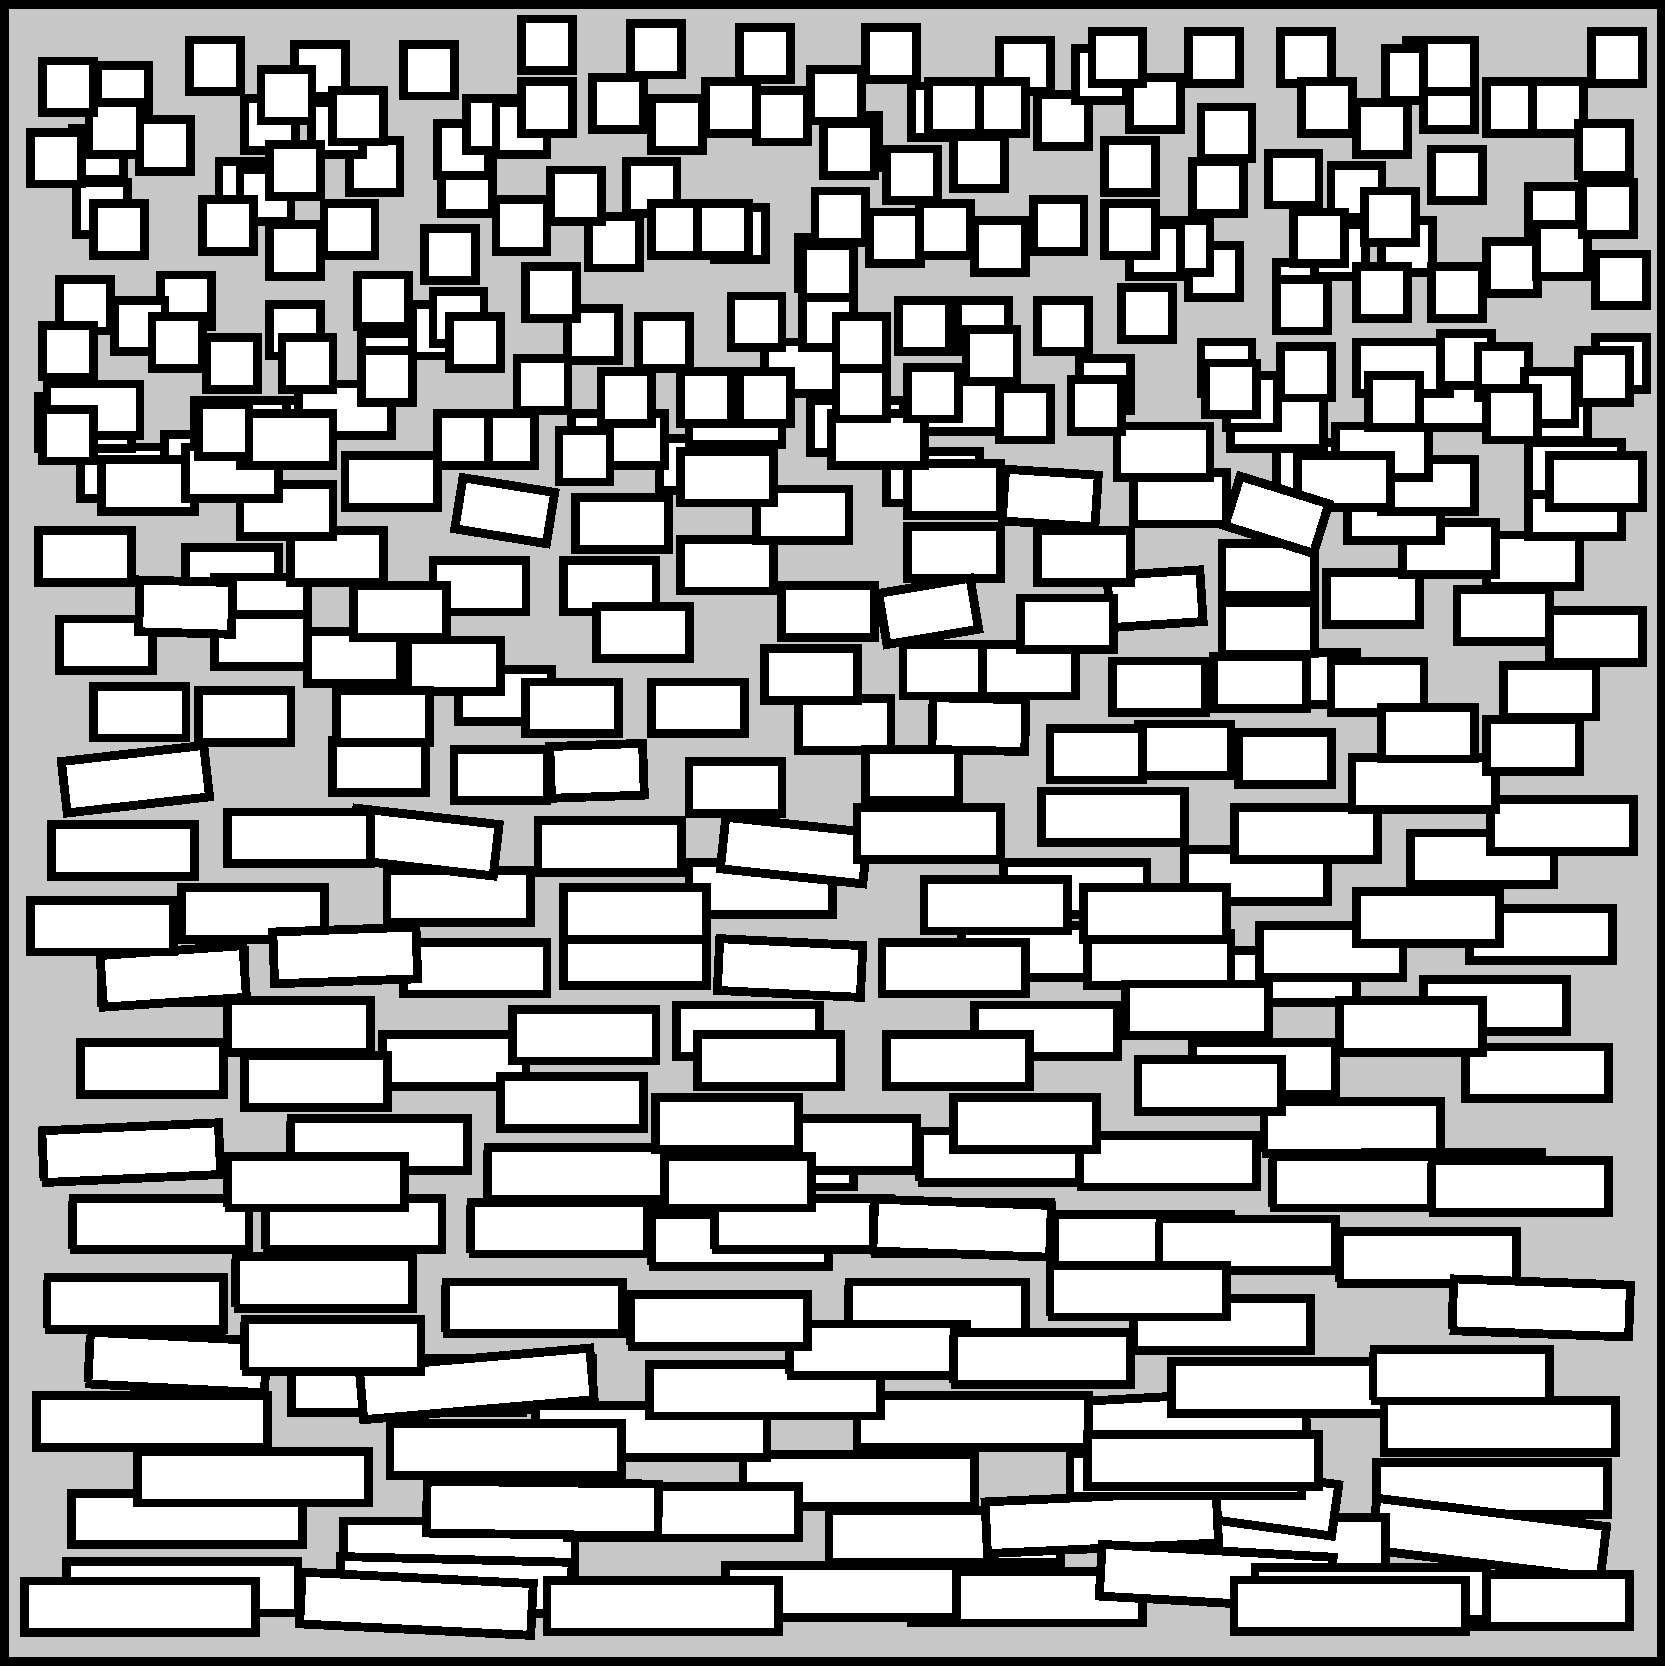
\includegraphics[width=0.2\textwidth]{figures/introduction/twist}}\hspace{0.2cm}
\subfigure[Bend]{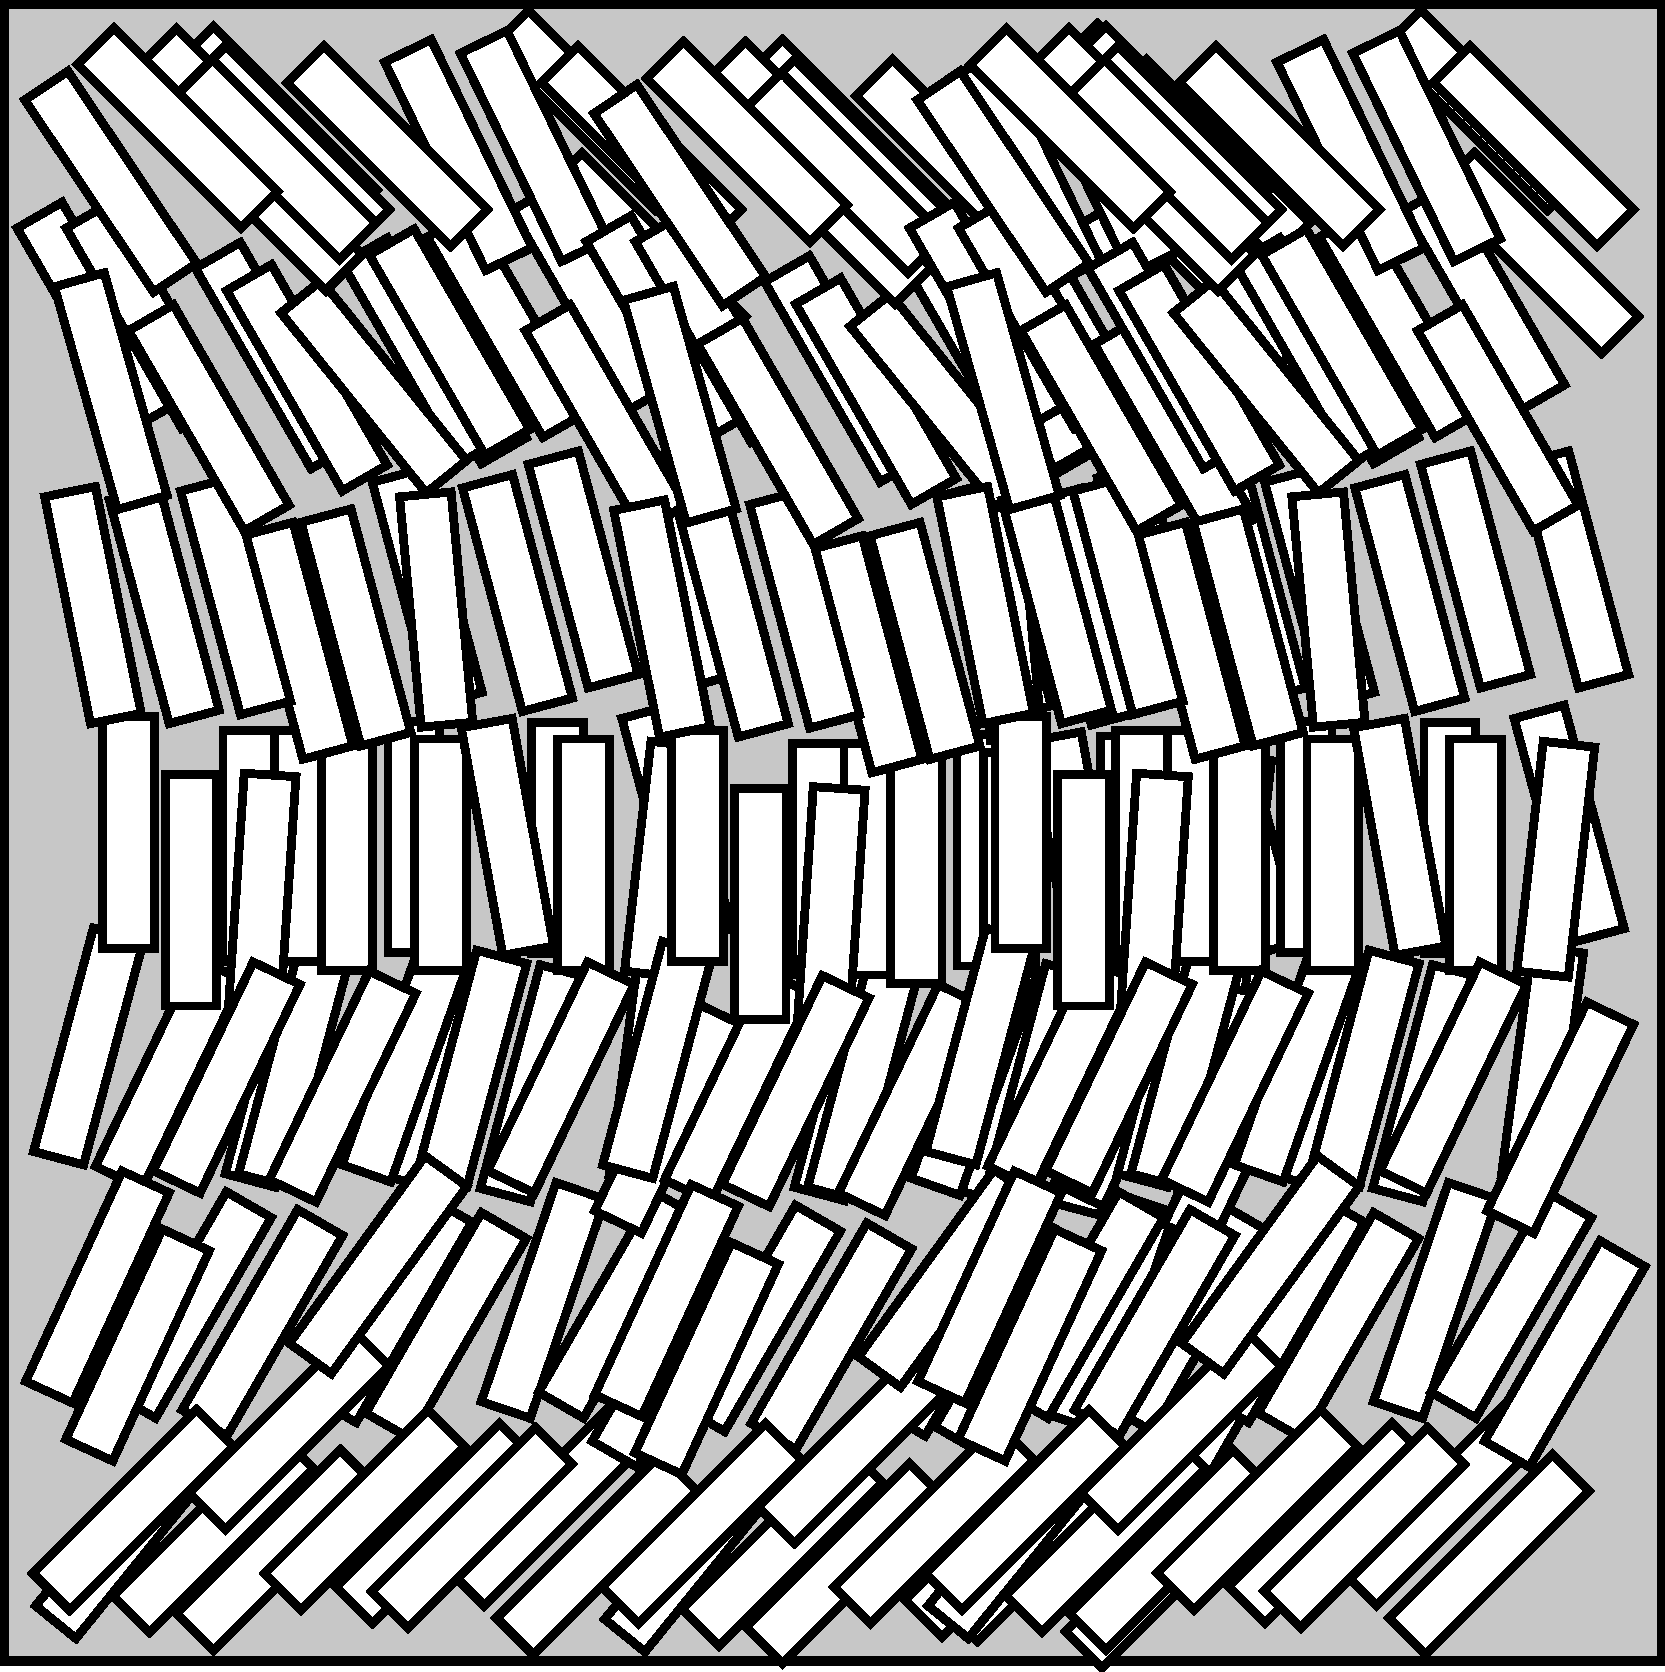
\includegraphics[width=0.2\textwidth]{figures/introduction/bend}}\hspace{0.2cm}
\end{center}
\caption[Schematic depiction of the splay, twist and bend elastic deformations]{\label{fig:s,t,b}A schematic diagram of the elastic deformations that can be imposed on a nematic liquid crystal via application of boundary conditions, (a) splay, (b) twist and (c) bend. Each white rectangle represents a nematic liquid crystal molecule. For the twist deformation (b), the director is rotating through 90$^{\circ}$ from the bottom surface to the top surface.}
\end{figure}



\begin{equation}
\frac{1}{2}\left(k_{22}+k_{24}\right)\nabla.\left(\bm{n}.\nabla\bm{n}-\bm{n}\nabla.\bm{n}\right)
\end{equation}

The free energy density expression for a non-chiral nematic does not include this term because the undistorted state is exactly the same as uniform alignment. The chirality of the molecules in a chiral nematic sample introduces an extra twist term between the intermolecular interactions.

\subsection{Surface alignment}
For efficient operation of nearly all liquid crystal devices, a well ordered and uniformly aligned mono-domain of the nematic director is required. In order to create uniform areas of alignment, the director can be forced to exhibit a specific direction relative to the cell wall by the application of a thin alignment layer, most commonly a spin-coated polyimide layer. 

\begin{figure}
\begin{center}
\subfigure[Planar]{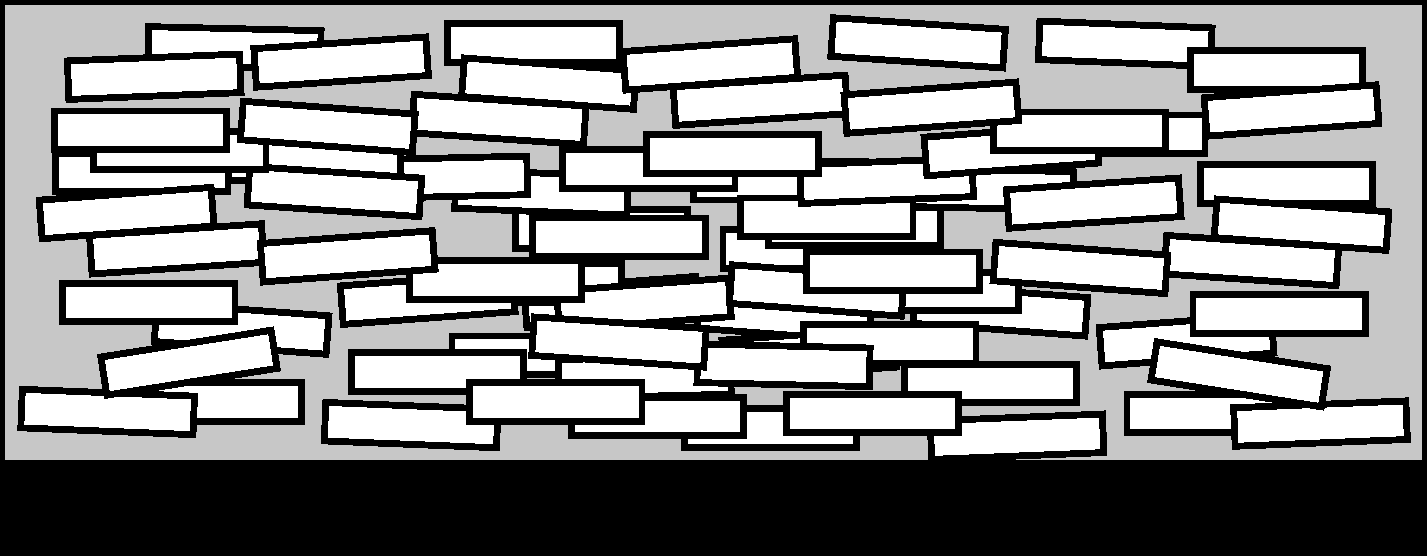
\includegraphics[width=0.2\textwidth]{figures/introduction/planar}}
\subfigure[Vertical]{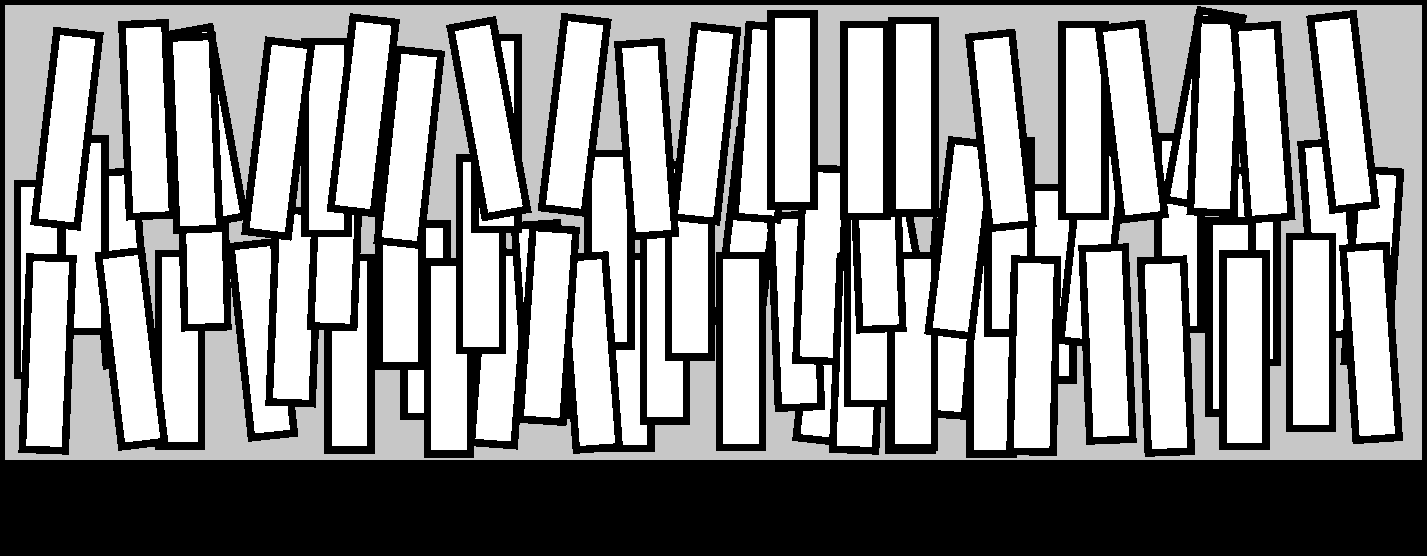
\includegraphics[width=0.2\textwidth]{figures/introduction/vertical}}
\subfigure[Tilted]{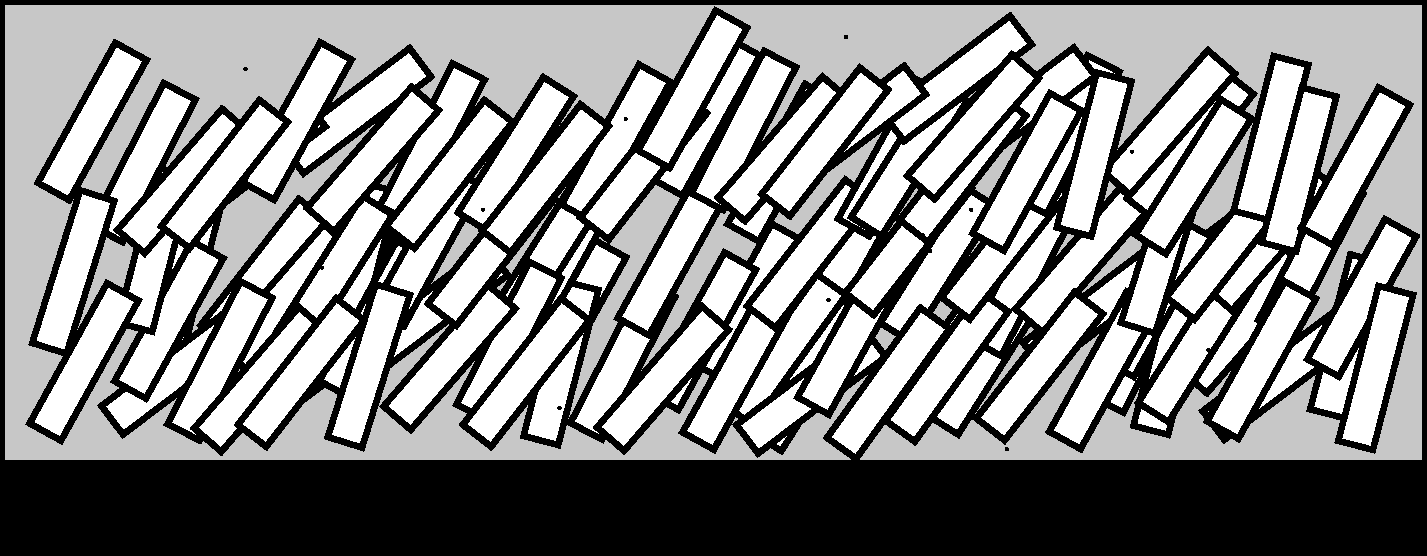
\includegraphics[width=0.2\textwidth]{figures/introduction/tilted}}
\end{center}
\caption[Schematic depiction of planar, vertical and tilted alignment]{\label{fig:alignment}Figures (a - c) depict schematic representations of planar, vertical and tilted alignment of the nematic director on a surface (black rectangle). Each white rectangle represents a nematic liquid crystal molecule.}
\end{figure}

Commonly required alignments are for the director to be planar homogeneous (parallel to the surface, at any azimuthal angle), vertical (parallel to the surface-normal, also sometimes termed homeotropic alignment) and tilted alignment (any angle between planar and vertical). These alignment states are schematically depicted in Figure \ref{fig:alignment} (a), (b) and (c). It is also not uncommon to promote different alignment of the director on multiple surfaces of the same device. Such alignments can force large gradients in $\hat{\bm{n}}$ in a stable state, thus creating non-zero values of the free energy (equation \ref{eq:Free_energy}). A much more detailed examination of surface alignment techniques and methods is discussed in Chapter \ref{cha:pretilt}.

\subsection{Nematic viscosities}
Unlike regular isotropic fluids, nematic liquid crystals also exhibit anisotropic viscosity. That is, the viscosity (constant of proportionality between the applied sheer stress and the induced velocity gradient) varies depending on the alignment of the director relative to the flow direction.
The first accurate determination of these anisotropic viscosities in nematics was carried out by Professor Marian Miesowicz in the 1930s (originally published in a small bulletin in German), but was not reported wide-spread until after the war in 1946 \cite{Miesowicz1946}. In his experiments, Miesowicz was able to distinguish three principal viscosity coefficients\footnote{For the liquid crystal PPA at 122$^{\circ}$ C (in the nematic phase)} $\left(\eta_{1,2,3}\right)$, shown schematically in Figure \ref{fig:eta} through the application of a strong magnetic field used to align the director in different orientations relative to the flow direction.

\begin{figure}
\begin{center}
\subfigure[$\eta_1$]{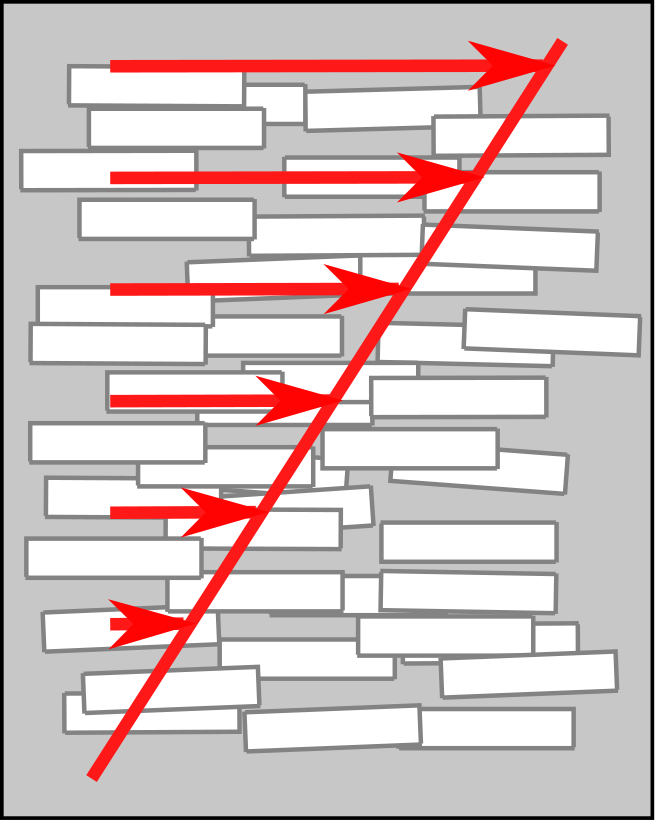
\includegraphics[width=0.15\textwidth]{figures/introduction/eta1.png}}
\subfigure[$\eta_2$]{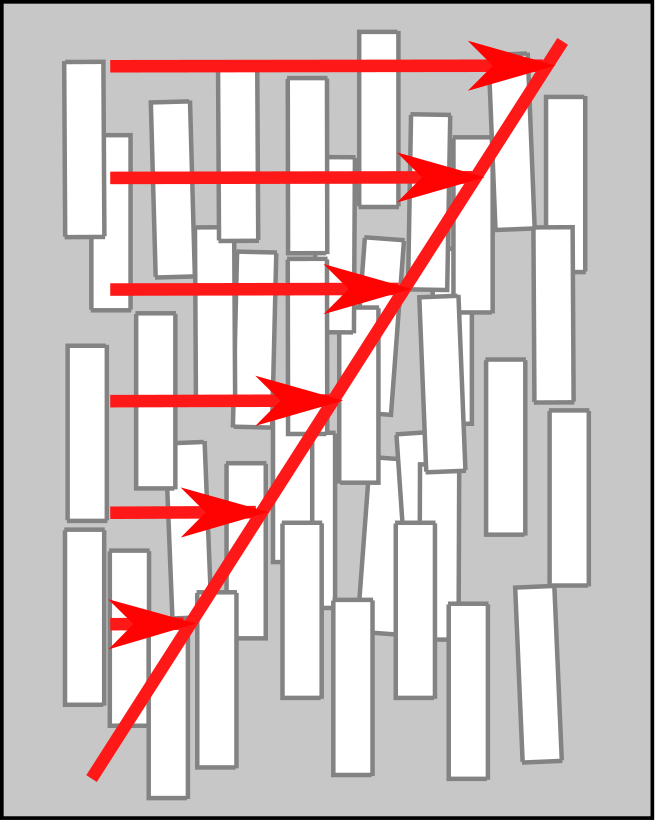
\includegraphics[width=0.15\textwidth]{figures/introduction/eta2.png}}
\subfigure[$\eta_3$]{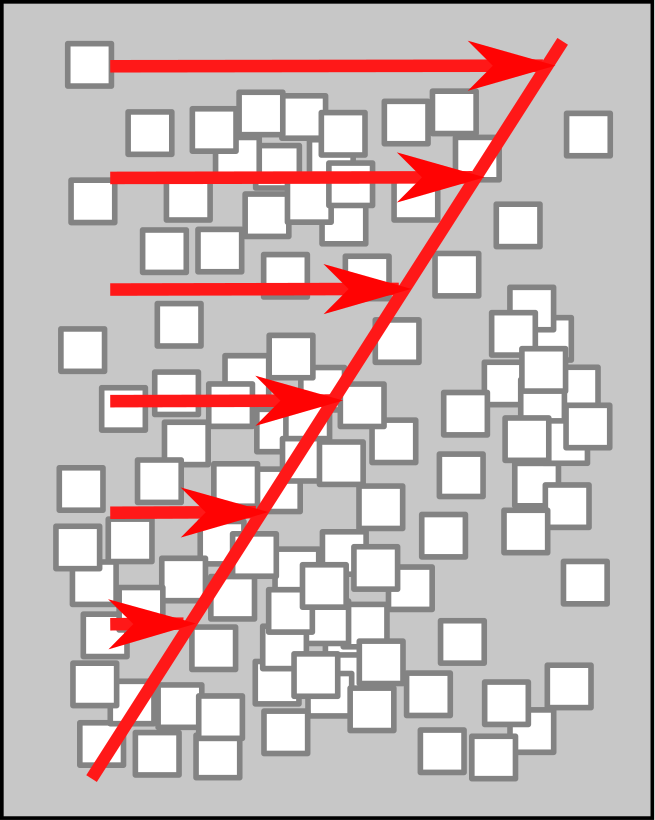
\includegraphics[width=0.15\textwidth]{figures/introduction/eta3.png}}
\end{center}
\caption[Caption]{\label{fig:eta}A schematic diagram representing the relationship between the flow direction (red arrows) and the alignment of the director for the principal Miesowicz viscosities, $\eta_1,\eta_2,\eta_3$}
\end{figure}

As is shown in Figure \ref{fig:eta}, the three principal Miesowicz viscosities correspond to three orientations of the director relative to the flow direction\footnote{The notation adopted here is the notation used by Miesowicz, but some texts adopt the Helfrich notation \cite{Helfrich1969a} which interchanges the above definitions of $\eta_1$ and $\eta_2$.},

\begin{enumerate}
\item $\eta_1$ when $\bm{n}$ is parallel to $\bm{v}$
\item $\eta_2$ when $\bm{n}$ is parallel to $\nabla\bm{v}$
\item $\eta_3$ when $\bm{n}$ is orthogonal to both $\bm{v}$ and $\nabla\bm{v}$
\end{enumerate}

It is worth noting that as quoted in Janik's scientific appreciation of Miesowicz' work on the anisotropic viscosities of liquid crystals, `\textit{...the accuracy of Miesowicz' experiments was so good that no significant improvement has been reported until the present time.}' \cite{Janik1992}. The results of this experiment are perhaps made even more significant when one considers that during the 1930s it was a generally accepted paradigm that that the properties of liquids were isotropic. As such, Miesowicz' results were originally met with some speculation from his contemporaries \cite{Janik1992}.
Values for the Miesowicz viscosities of 5CB near 25 $^{\circ}$C are given as $\eta_1=0.0204 \text{ Pa s},\eta_2=0.1052 \text{ Pa s},\eta_3=0.0326 \text{ Pa s}$ \cite{Stewart2004}.

As will be expanded upon in the next chapter, consideration of the full viscous stress tensor leads to the definition of not only the three principal Miesowicz viscosities as detailed above, but rather five independent viscosity coefficients for nematics. These viscosities cannot be related to the orientation of the director in a simple experimental manner \cite{Stewart2004} as is shown in Figure \ref{fig:eta} but rather occur in linear combinations, making visualisation of nematic viscosities very difficult. As will be seen later, the five independent nematic viscosities can be mathematically related to the Miesowicz viscosities.
